\section{Introduction}\label{sec:introduction}

As the world is becoming more connected and instrumented, we are receiving an increasing rate of digital information in the form of continuous data streams. Financial markets, telecommunications, manufacturing systems and health care systems are just a few examples of sources of continuous data streams. The data produced by these systems need to be analyzed in near real time to extract valuable information and take automated actions promptly. 

Stream processing systems process continuous data streams in an on-the-fly manner, as the data flows through the system. Their data processing paradigm represent the computation as a graph of operators and streams, where operators are generic data manipulators and streams are connections between operators. As long as they manage to cope with high data rates, they are a good fit for online data analytics tasks. 

A few characteristics of stream processing systems have a significant effect on how they perform their tasks. First, they are long-running applications. Once deployed, they should perform their task continuously for a long time without any interruption. Secondly, rate of the data in continuous streams are highly dynamic. Therefore, they must perform performance optimizations to adapt to their workload changing during their lifetime. 

In this study, we are researching new techniques to implement a distributed stream processing engine that can adapt to its dynamic workload with the capability of changing all aspects of all logical-to-physical mapping at runtime with reasonable cost. We call this capability \textit{organic adaptation}. It will have three important properties that will form a trivet (TODO corner stone???) for its adaptation capabilities:
\begin{itemize}
\item An integrated solution that can perform multiple optimizations (TODO list these optimizations) at runtime with little overhead, considering their interactions with each other.
\item Runtime utilities to perform changes on configurations and logical-to-physical mappings resiliently with little overhead.
\item An operator development API that enables users to implement their generic, reusable operators easily, Additionally, this API should enable users to provide information about operator properties such that stream processing engine will understand behavior of the operator and perform optimizations safely, and efficiently.

\end{itemize}

This is a reference to a Section~\ref{sec:related}.

This is a reference to a Figure~\ref{fig:bugra1}.

This is a reference to a Table~\ref{tbl:data}.

This is a bib reference~\cite{ref:SPL}.

\begin{figure*}[t]
\centering
\begin{minipage}{0.48\linewidth}
  \centering
  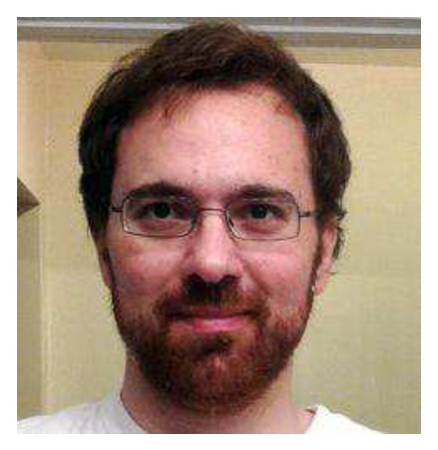
\includegraphics[width=0.5\linewidth]{figures/bugra.eps}
  \caption{Caption goes here}\label{fig:bugra1}
\end{minipage}
\vspace{0.01\linewidth}
\begin{minipage}{0.48\linewidth}
  \centering
  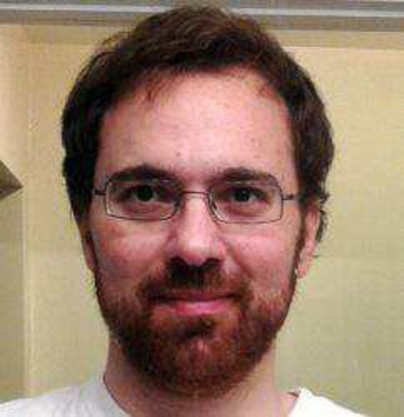
\includegraphics[width=0.5\linewidth]{figures/bugra.pdf}
  \caption{Caption goes here}\label{fig:bugra2}  
\end{minipage}
\end{figure*}


\begin{table*}[t]
\centering
\begin{tabular}{|l||c|c|c|}\hline 
\emph{props.}$\backslash$\emph{names} 
              & seqNo    & RIC     & Date         \\\hline
types         & long     & string  & string       \\\hline
sizes         & $0.08$   & $0.07$  & $0.15$       \\\hline
best alg.     & seq      & zlib    & sameVal      \\\hline
compr. ratios & $\sim 0$ & $0.28$  & $\sim 0$     \\\hline
compr. cost   & $0.006$  & $0.224$ & $0.006$      \\\hline
compr. rank   & $0$      & $7$     & $1$          \\\hline
\end{tabular}
\caption{Properties of the attributes in the TAQ data set.}\label{tbl:data}
\end{table*}            

